\documentclass[acmlarge,review]{acmart}\settopmatter{printfolios=true}

\usepackage{amssymb}
\usepackage{amsthm}
\usepackage{graphicx}
\usepackage{amsmath}
\usepackage{mathptmx}
\usepackage{mathtools}
\usepackage{stmaryrd}
\usepackage{hyperref}
\usepackage{alltt}
\usepackage{url}
\usepackage{float}
\usepackage{style/utils}
\usepackage{style/code}
\usepackage{style/proof}
\usepackage{style/keywords}
\usepackage{style/layout}
\usepackage{style/judgements}

% for combinator pictures
\usepackage{tikz}
\usetikzlibrary{shapes,arrows}
\usepackage[outputdir={out/}]{dot2texi}

\setcopyright{none}
\bibliographystyle{ACM-Reference-Format}
\citestyle{acmauthoryear}

% -----------------------------------------------------------------------------
\begin{document}

\title{Machine fusion}
\subtitle{Merging merges, more or less}

\author{Amos Robinson}
\affiliation{UNSW (Australia)}
\email{amosr@cse.unsw.edu.au}

\author{Ben Lippmeier}
\affiliation{Digital Asset and UNSW (Australia)}
\email{benl@ouroborus.net}

\makeatactive
\begin{abstract}
Compilers for stream programs often rely on a fusion transformation to convert the implied data-flow network into low-level iteration based code. Different fusion transformations handle different sorts of networks, with the distinguishing criteria being whether the network may contain splits and joins, and whether the set of fusible operators can be extended. We present the first fusion system that simultaneously satisfies all three of these criteria: networks can contain splits and joins, and new operators can be added to the system without needing to modify the overall fusion transformation. Our system has been formalized in Coq, and we have proved soundness of the core transformation.
\end{abstract}


\maketitle

%!TEX root = ../Main.tex
\section{Introduction}

Data flow fusion~\cite{lippmeier2013flow} is a technique to compile a specific class of data flow programs into single, efficient imperative loops. This process of ``compilation'' is equivalent to performing array fusion on a combinator based functional array program, as per related work on stream fusion~\cite{coutts2007streamfusion} and delayed arrays~\cite{keller2010repa}. The key benefits of data flow fusion over this prior work are: 1) it fuses programs that use branching data flows where a produced array is consumed by several consumers, and 2) complete fusion into a single loop is guaranteed for all programs that operate on the same size input data, and contain no fusion-preventing dependencies between operators.

Fusion-preventing dependencies express the fact that some operators simply must wait for others to complete before they can produce their own output. For example, in the following:
\begin{code}
  normalize :: Array Int -> Array Int
  normalize xs = let sum = fold (+) 0 xs
                 in  map (/ sum) xs
\end{code}

If we wish to divide every element of an array by the sum of all elements, then it seems we are forever destined to compute the result using at least two loops: one to determine the sum, and one to divide the elements. The evaluation of @fold@ demands all elements of its source array, and we cannot produce any elements of the result array until we know the value of @sum@. 

However, many programs \emph{do} contain opportunities for fusion, if we only knew which opportunities to take. The following example offers \emph{several} unique, but mutually exclusive approaches to fusion. Figure~\ref{f:normalize2-cluterings} on the next page shows some of the possibilities.
\begin{code}
 normalize2 :: Array Int -> Array Int
 normalize2 xs
  = let sum1 = fold   (+)  0   xs
        gts  = filter (> 0)    xs
        sum2 = fold   (+)  0   gts
        ys1  = map    (/ sum1) xs
        ys2  = map    (/ sum2) xs
    in (ys1, ys2)
\end{code}

In Figure~\ref{f:normalize2-cluterings}, the dotted lines show possible clusterings of operators. Stream fusion implicitly choses the solution on the left as its compilation process cannot fuse a produced array into multiple consumers. The best existing ILP approach will chose the solution on the right as it cannot cluster operators that consume arrays of different lengths. Our system choses the solution in the middle, which is also optimal for this example. 

% NOTE: This set of bullets needs to fit on the first page, without spilling to the second.
Our contributions are as follows:
\begin{itemize}
\item   
We extend prior work by Megiddo~\cite{megiddo1998optimal} and Darte~\cite{darte2002contraction}, with support for length changing operators. Length changing operators can be clustered with the operators that generate their source arrays, and compiled naturally with data-flow fusion (\S\ref{s:ILP}).

\item
We present a simplification to constraint generation that is also applicable to some existing integer linear programming formulations such as Megiddo's,
where constraints between two nodes need not be generated if there exists a fusion-preventing path between the two (\S\ref{s:OptimisedConstraints}).

\item
Our constraint system also encodes a total ordering on the cost of clusterings, expressed using weights on the integer linear program. For example, we encode that memory traffic is more expensive than loop overheads, so given a choice between the two, the memory traffic will be reduced (\S\ref{s:ObjectiveFunction}).

\item
We present benchmarks of our algorithm applied to several common programming patterns, and to several pathological examples.
Our algorithm is complete and yields good results in practice, though if array sizes are unknown, an optimal solution is uncomputable in general. \TODO{ref}
\end{itemize}

The reduction of the clustering problem to integer linear programming was previously described by~\cite{megiddo1998optimal}, though they do not consider length changing operators.


% We must also decide which clustering is the `best' or most optimal. One obvious criterion for this is the minimum number of loops, but there may even be multiple clusterings with the minimum number of loops. In this case, the number of required manifest arrays must also be taken into account. 

% As real programs contain tens or hundreds of individual operators, performing an exhaustive search for an optimal clustering is not feasible, and greedy algorithms tend to produce poor solutions. 


%!TEX root = ../Main.tex
\section{Processes, Machines, Combinators and Operators}
\label{s:Processes}

A \emph{process} in our system is a simple imperative program with a local heap. A process pulls data from an arbitrary number of input streams and pushes result values to at least one output stream. The process language is an intermediate representation we use when fusing the overall dataflow network. When describing the fusion transform we describe the control flow of the process as a state machine, hence Machine Fusion. 

A \emph{combinator} is a template for a particular process which parameterises it over the particular input and output streams, as well as values of configuration parameters such as the worker function used in a @map@ process. Each process implements a logical \emph{operator} --- so we use ``operator'' when describing the values being computed, but ``process'' and ``machine'' when referring to the implementation. 


% -----------------------------------------------------------------------------
\subsection{Grouping}

The definition of the @group@ combinator which removes consecutive elements from its input stream is given in Fig.~\ref{fig:Process:Group}. We include the concrete code representation and a diagram of the process viewed as a state machine.

The @group@ combinator has two parameters, @sIn1@ and @sOut1@, which bind the input and output streams respectively. The \emph{nu-binders} \mbox{$\nu$ @(f: Bool) (l: Nat)@...} indicate that each time the @group@ combinator is instantiated, fresh names must be given to @f@, @l@ and so on, that do not conflict with other instantiations. 

The body of the combinator is a record that defines the process. The @ins@ field of the record defines the set of input streams and the @outs@ field the set of output streams. The @heap@ field gives the initial values of each of the local variables. The @instrs@ field contains a set of labeled instructions that define the program, while the @label@ field gives the label of the initial instruction. 

The initial instruction @(pull sIn1 v A1 {})@ pulls the next element from the stream @sIn1@, writes it into the heap variable @v@ (value), then proceeds to the instruction at label @A1@. The empty set @{}@ after the target label @A1@ can be used to update values in the heap, but as we do not need to update anything yet we leave it empty. 

Next, the instruction @(case (f || (l /= v)) A2 {} A3 {})@ checks whether predicate @(f || (l /= v))@ is true; if so it proceeds to the instruction at label @A2@, otherwise it proceeds to @A3@. We use the variable @l@ (last) to track the last value read from the stream, and the boolean @f@ (first) for whether this is the first element.

When the predicate is true, the instruction @(push sOut1 v A3 { l = v, f = F })@ pushes the value @v@ to the output stream @sOut1@ and proceeds to the instruction at label @A3@, once the heap has been updated to set variable @l@ to @v@ and @f@ to @F@ (False). 

Finally, the instruction @(drop sIn1 A0 {})@ signals that the current element that was pulled from stream @sIn1@ is no longer required, and goes back to the first the instruction at @A0@. This @drop@ instruction is used to coordinate concurrent processes when performing fusion. The next element of a stream may only be pulled after all consumers have pulled and then and dropped the current element.

Overall, the @f@ variable tracks whether we are dealing with the first value from the stream, @l@ holds the last value pulled from the stream (or 0 if none have been read yet), and @v@ holds the current value pulled from the stream. The process emits the first value pulled from the stream and every value that is different from the last one that was pulled. For example, when executed on the input stream $[1, 2, 2, 3]$, the process will produce the output $[1, 2, 3]$.

\begin{figure}

\begin{center}
\begin{alltt}
           group 
             = \(\lambda\) (sIn1: Stream Nat) (sOut1: Stream Nat). 
               \(\nu\) (f: Bool) (l: Nat) (v: Nat) (A0..A3: Label).
\end{alltt}
\begin{code}
               process
               { ins:    { sIn1  }
               , outs:   { sOut1 }
               , heap:   { f = T, l = 0, v = 0 }
               , label:  A0
               , instrs: { A0 = pull sIn1 v          A1 {}
                         , A1 = case (f || (l /= v)) A2 {}  A3 {}
                         , A2 = push sOut1 v         A3 { l = v, f = F }
                         , A3 = drop sIn1            A0 {} } }
\end{code}
\end{center}
\vspace{1em}
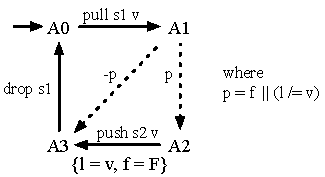
\includegraphics[scale=1.1]{figures/state-group.pdf}
\caption{The group combinator}
\label{fig:Process:Group}
\end{figure}


% -----------------------------------------------------------------------------
\subsection{Merging}
\begin{figure}
\begin{alltt}
               merge
                 = \(\lambda\) (sIn1: Stream Nat) (sIn2: Stream Nat) (sOut2: Stream Nat). 
                   \(\nu\) (x1: Nat) (x2: Nat) (B0..E2: Label).
\end{alltt}
\begin{code}
                   process
                   { ins:    { sM1, sM2 }
                   , outs:   { sM3 }
                   , heap:   { x1 = 0, x2 = 0 }
                   , label:  B0
                   , instrs: { B0 = pull sIn1  x1   B1 {}
                             , B1 = pull sIn2  x2   C0 {}
                             , C0 = case (x1 < x2)  D0 {}  E0 {}
                             , D0 = push sOut2 x1   D1 {}
                             , D1 = drop sIn1       D2 {}
                             , D2 = pull sIn1  x1   C0 {}
                             , E0 = push sOut2 x2   E1 {}
                             , E1 = drop sIn2       E2 {}
                             , E2 = pull sIn2 x2    C0 {} } }
\end{code}

\medskip
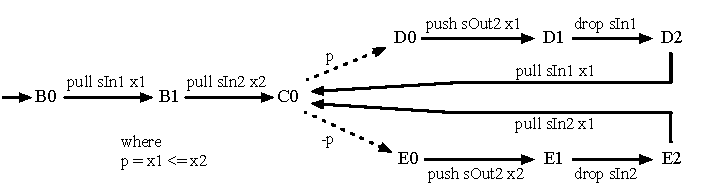
\includegraphics[scale=1.1]{figures/state-merge.pdf}
\caption{The merge combinator}
\label{fig:Process:Merge}
\end{figure}

The definition of the @merge@ combinator, which merges two input streams, is given in Fig.~\ref{fig:Process:Merge}. The combinator binds the two input streams to @sIn1@ and @sIn2@, while the output stream is @sOut2@. The two heap variables @x1@ and @x2@ are used to store the last values read from each input stream. The process starts by pulling from each input streams. It then compares the two pulled values, and pushes the smaller of the values to the output stream. The process then drops the stream which yielded the the smaller value, then pulls from the same stream so that it can perform the comparison again.

As this process merges infinite streams, if we execute it with a finite input prefix, it will arrive at an intermediate state that may not yet have pushed all available output. For example, if we execute the process with the input streams $[1, 4]$ and $[2, 3, 100]$ then the values $[1, 2, 3, 4]$ will be pushed to the output.
After pushing the last $4$, the process will block at instruction @E2@, waiting for the next value to be pulled from @sIn2@. We discuss how to handle finite streams later in ~\S\ref{s:Finite}.


% -----------------------------------------------------------------------------
\subsection{Fusion}
Our fusion algorithm takes two process state machines and produces a new one that computes the outputs of both. For example, suppose we need a single machine that computes the outputs of the first two combinators of our @uniquesUnion@ example back in \S\ref{s:Introduction}. The result will be a machine that computes the result of both the @group@ and @merge@ if they were executed concurrently, where the first input stream of the @merge@ is the same as the input stream of the @group@. For ease of comparison we will assume the parameters in each combinator are instantiated by arguments with the same names.


% -----------------------------------------------------------------------------
\subsubsection{Fusing Pulls}

The algorithm proceeds by considering pairs of states: one in each of the machines to be fused. Both the @group@ machine and the @merge@ machine pull from the same stream as their initial instruction, so we have the situation shown in Fig.~\ref{fig:Fusion:Pulls}. The @group@ machine needs to transition from label @A0@ to label @A1@, and the @merge@ machine from @B0@ to @B1@. In the result machine we produce three new instructions that transition between four result states, @F0@ to @F3@.
Each of the result states represents a combination of two original states, one from each of the input machines. For example, the first result state @F0@ represents a combination of the @group@ machine being in its initial state @A0@ and the @merge@ machine being in its own initial state @B0@. 

We also associate each of the result states with information describing whether or not each machine has already pulled a value from each input stream. For the @F0@ case shown in Fig.~\ref{fig:Fusion:Pulls} we have ((A0, \{sIn1 = none\}), (B0, \{sIn1 = none, sIn2 = none\})). The result state @F0@ represents a combination of the two input states @A0@ and @B0@. As both @A0@ and @B0@ are the initial states of their respective machines, those machines have not yet pulled any values from their two input streams, so both @sIn1@ and @sIn2@ map to `none'.

From the joint state @F0@, both of the input machines then need to pull from stream @sIn1@, the @group@ machine storing the value in a variable @v@ and the @merge@ machine storing it in @x1@. In the result machine this is managed by storing the pulled value in a fresh buffer variable @b1@, and then using later instructions to copy the value into the original variables @v@ and @x1@. For this we use the @jump@ instruction which transitions between states without affecting any of the input or output streams.


Finally, note that in the result states @F0@ through @F3@ the state of the input streams transitions from `none', to `pending' then to `have'. The `none' state means that we have not yet pulled a value from the associated stream. The `pending' state means we have pulled a value into the stream buffer variable (@b1@ in this case). The `have' state means that we have copied the pulled value from the stream buffer variable into the local variable used by each machine. In Fig.~\ref{fig:Fusion:Pulls},  `sIn1' is set to `have' for the first machine in @F2@ after we have set `v = b1', while `sIn1' is set to `have' for the second machine in @F3@ after we have set `x1 = b1'. 


\begin{figure}
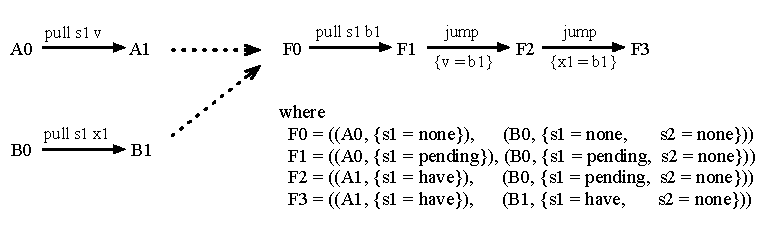
\includegraphics[scale=1.1]{figures/fuse-pull-pull.pdf}
\caption{Fusing pull instructions}
\label{fig:Fusion:Pulls}
\end{figure}


% -----------------------------------------------------------------------------
\subsubsection{Fusing Cases}
\begin{figure}
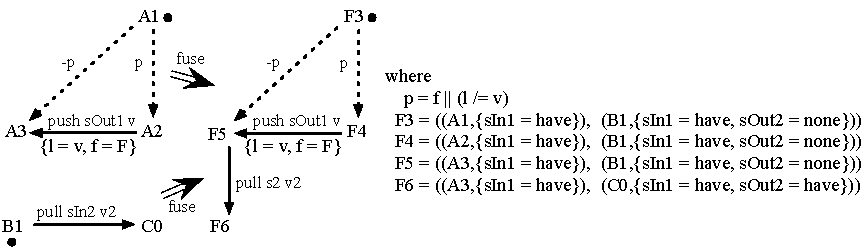
\includegraphics[scale=1.1]{figures/fuse-case-pull.pdf}
\caption{Fusing case instructions}
\label{fig:Fusion:Case}
\end{figure}

Once the result machine has arrived in the joint state @F3@, this is equivalent to the two input machines arriving in states @A1@ and @B1@ respectively.
Fig.~\ref{fig:Fusion:Case} shows the next few transitions of these machines.
From state @A1@, the @group@ machine needs to perform a @case@ branch to determine whether to push the current value it has from its input stream @sIn1@ to its output stream @sOut1@, or to just move on to the next value from its input. From state @B1@, the @merge@ machine needs to pull a value from its second input stream @sIn2@. In the result, @F3@ performs the case analysis from @A1@, moving to either @A2@ or @A3@, corresponding to @F4@ and @F5@ respectively.
At @F4@, the push at @A2@ is executed and moves to @A3@, corresponding to @F5@.

Finally, at @F5@ the @merge@ machine pulls from @sIn2@, moving from @B1@ to @C0@.
Because the stream @sIn22@ is only pulled from by the @merge@ machine, no coordination is required between @merge@ and @group@ for this pull.

Note that we could construct the fused machine in multiple ways. One option is to perform the case branch first and then pull from @sIn2@, another is to pull from @sIn2@ first and then perform the branch. By construction, the predicate used in the branch only refers to variables local to the @group@ machine, and the pull instruction from @B1@ stores its result in a variable local to the @merge@ machine. As the set of variables does not overlap, either ordering is correct. For this example we choose to perform the branch first, though will discuss the ramifications of this choice further in \S\ref{s:FusionOrder}. 


% -----------------------------------------------------------------------------
\subsection{Fused Result}

Fig.~\ref{fig:Process:Fused} shows the entire result of fusing @group@ and @merge@ together. There are other rules for handling different combinations of instructions, but we defer the details to \S\ref{s:Fusion}. The result process has two inputs, @sIn1@ and @sIn2@, which correspond to the original input streams. Of the two outputs, @sOut1@ is the @group@ processes output stream, while @sOut2@ is the @merge@ processes output stream. 

Overall, our fusion algorithm has taken two separate processes that we once imagined to be running concurrently, and has produced a single sequental result process that implements both. We have chosen a \emph{specific sequential order} in which to interleave instructions that implement both original processes. As with the Flow Fusion system of \cite{lippmeier2013data} we have performed the job of a concurrent scheduler at compile time. However, in contrast to Flow Fusion and similar systems, we do not need to organize statements into a fixed \emph{loop anatomy}, we simply merge them as they are. This allows us to implement a wider range of processes, including ones with nested loops that work on segmented streams, which we discuss further in \S\ref{s:FutureWork}. 

To complete the implementation of our example from \S\ref{s:Introduction} we would now proceed to fuse the process from the final line (also a @group@) into this new result process. The order in which processes are fused together does matter, as does the order in which the instructions are emitted --- we discuss both points further in \S\ref{s:Evaluation}.

Finally, although the result process has a single shared heap, the bindings are guaranteed not to interfere. When we instantiate combinators to create the original processes we use fresh names at that point. The stream buffer variables we aditionally introduce for coordination are freshly created during fusion.


% BL: This is too much low level detail at this point, we need more intuition.

% The instructions of @merge@ can be split into four categories, which can be identified in the fused process: labels @B0@-@B2@ perform initialisation, and are mapped to @F0@-@F6@; label @C0@ performs case analysis to find the smaller value and is mapped to @F7@; labels @D0@-@D2@ push the value from the first stream, @s1@, and are mapped to @F8@-@F15@; and labels @E0@-@E2@ push the value from the second stream, @s2@, and are mapped to @F16@-@F18@.

% The @group@ process can also be identified in the fused process: the fused labels @F0@-@F5@ perform the pulling, case analysis and pushing from instructions @A0@-@A2@. These instructions are seen again in @F10@-@F14@, when the @merge@ process is pulling from the @s1@ stream. Thus the @group@ instructions have been duplicated, and are performed once when @merge@ initialises, and again every time @merge@ pulls from the first stream.

% Labels @F5@ and @F14@ correspond to the (@drop s1@) instruction at @A3@ in @group@, but note that they are fused as @jump@ instructions. As @s1@ is shared between the two processes, the element from @s1@ can only be dropped once both processes agree to drop. In the fused labels on the right hand column, the other process still has @s1@ as `pending' or `have', so the element cannot yet be dropped. The actual @drop@ is only performed once both processes are `none', at label @F9@.
 

\begin{figure}
\begin{code}
process
{ ins:    { sIn1,  sIn2 }
, outs:   { sOut1, sOut2 }
, heap:   { f = T, l = 0, v = 0, x1 = 0, x2 = 0, b1 = 0}
, label:  F0
, instrs:
\end{code}

\newcommand\annot[5]{
  \tiny ((#1,   \> \tiny \{sIn1 =      #2\}), 
                \> \tiny (#3, \> \tiny \{sIn1 =      #4, \> \tiny sIn2 =      #5\}))
}
\newcommand\icase[7]{
 \tt{#1} \> \tt{= #2} \> \tt{#3} \{\tt{#4}\} \> \tt{#5} \{\tt{#6}\} \> \tiny #1 \> \tiny = #7 \\
}
\newcommand\instr[5]{
 \tt{#1}\>\tt{= #2} \> \tt{#3} \{\tt{#4}\} \> \> \tiny #1 \> \tiny = #5 \\
}
\begin{tabbing}
@  @ \=
@, F17@  \= = @case (f || (l /= v)) @
         \= @F17{x1 = b1, f = F}@ \= @F17{ }@
@      @ \= \tiny F17 \= \tiny = ((A0, \= \tiny \{s1 = pending\}), \= \tiny (B0, \= \tiny \{s1 = pending, \= \tiny s2 = pending\})) \kill
\> @{@ \instr{F0}{pull sIn1 b1}{F1}{}
      {\annot{A0}{none}{B0}{none}{none}}

\> @,@
\instr{F1}{jump}{F2}{v  = b1}
      {\annot{A0}{pending}{B0}{pending}{none}}
\> @,@
\instr{F2}{jump}{F3}{x1 = b1}
      {\annot{A1}{have}{B0}{pending}{none}}
\> @,@
\icase{F3}{case (f || (l /= v))}{F4}{}{F5}{}
      {\annot{A1}{have}{B1}{have}{none}}

\> @,@
\instr{F4}{push sOut1 v}{F5}{l = v, f = F}
      {\annot{A2}{have}{B1}{have}{none}}

\> @,@
\instr{F5}{jump}{F6}{}
      {\annot{A3}{have}{B1}{have}{none}}

\> @,@
\instr{F6}{pull sIn2 x2}{F7}{}
      {\annot{A0}{none}{B1}{have}{none}}
\\

\> @,@
\icase{F7}{case (x1 < x2)}{F8}{}{F16}{}
      {\annot{A0}{none}{C0}{have}{have}}

\\
\> @,@
\instr{F8}{push sOut2 x1}{F9}{}
      {\annot{A0}{none}{D0}{have}{have}}
\> @,@
\instr{F9}{drop sIn1}{F10}{}
      {\annot{A0}{none}{D1}{none}{have}}
\> @,@
\instr{F10}{pull sIn1 b1}{F11}{}
      {\annot{A0}{none}{D2}{none}{have}}
\> @,@
\instr{F11}{jump}{F11}{v = b1}
      {\annot{A0}{pending}{D2}{pending}{have}}
\> @,@
\icase{F12}{case (f || (l /= v))}{F13}{}{F14}{}
      {\annot{A1}{have}{D2}{pending}{have}}
\> @,@
\instr{F13}{push sOut1 v}{F14}{l = v, f = F}
      {\annot{A2}{have}{D2}{pending}{have}}
\> @,@
\instr{F14}{jump}{F15}{}
      {\annot{A3}{have}{D2}{pending}{have}}
\> @,@
\instr{F15}{jump}{F7}{x1 = b1}
      {\annot{A0}{none}{D2}{pending}{have}}

\\
\> @,@
\instr{F16}{push sOut2 x2}{F17}{}
      {\annot{A0}{none}{E0}{have}{have}}
\> @,@
\instr{F17}{drop sIn2}{F18}{}
      {\annot{A0}{none}{E1}{have}{have}}
\> @,@
\instr{F18}{pull sIn2}{F7}{}
      {\annot{A0}{none}{E2}{have}{none}}

@} }@
\end{tabbing}

\caption{Fusion of group and merge}
\label{fig:Process:Fused}
\end{figure}









%!TEX root = ../Main.tex

\clearpage{}
\section{Process definitions}

%% This figure is referenced below, in 'Process definitions', but putting it up here before the big fused process stops the fused one from splitting across multiple pages.
%!TEX root = ../Main.tex

\begin{figure}
\begin{minipage}[t]{0.4\textwidth}
\begin{tabbing}
\Instr \TABDEF @MMMM@  \TABSKIP $\Exp$ \TABSKIP $\Exp$ \TABSKIP $\Exp$ \kill

\Exp,~$e$ \> $\to$ \> $x~|~v~|~e~e $ \\
  \> $\enskip|~$ \> $ (e~||~e) ~|~ e+e ~|~ e~@/=@~e ~|~ e < e$ \\
\Value,~$v$ \> $\to$ \> $\mathbb{N}~|~\mathbb{B}~|~(\lambda{}x.~e)$ \\
\Heap,~$\Sigma$ \> $\to$ \> $\cdot~|~\Sigma,~x~=~v$ \\
\\

\Proc \>:=\> @process@ \\
MMMMMM \= M \= \kill
\> \> @ins:   @  $(\Chan ~\mapsto~ \InputState)$ \\
\> \> @outs:  @  $\sgl{\Chan}$ \\
\> \> @heap:  @  \Heap \\
\> \> @label: @  \Label \\
\> \> @instrs:@  $(\Label ~\mapsto~ \Instr)$ \\
\\
\Instr \TABDEF \kill
\InputState \> := \> @none@~$|$~@pending@~\Value~$|$~@have@

\end{tabbing}
\end{minipage}
\begin{minipage}[t]{0.05\textwidth}
\quad
\end{minipage}
\begin{minipage}[t]{0.4\textwidth}
\begin{tabbing}
\Instr \TABDEF @MMMM@  \TABSKIP $\Chan$ \TABSKIP $\Chan$ \TABSKIP $\Exp$ \kill

\Var,~$x$ \> $\to$ \> (value variable) \\
\Chan,~$c$ \> $\to$ \> (channel/stream name) \\
\Label,~$l$ \> $\to$ \> (label name) \\
\\
\\

\Instr
    \> :=\> @pull@  \> \Chan  \> \Var  \> \Next \\
    \TABALT @push@  \> \Chan  \> \Exp  \> \Next \\
    \TABALT @case@  \> \Exp   \> \Next \> \Next \\
    \TABALT @jump@  \>        \>       \> \Next \\
    \TABALT @drop@  \> \Chan  \>       \> \Next \\
\\
\\
\Next \> := \> $\Label~\times~(\Var \mapsto \Exp)$ \\
\end{tabbing}
\end{minipage}
\caption{Process definitions}
\label{fig:Process:Def}
\end{figure}



The grammar for processes is shown in Fig.~\ref{fig:Process:Def}.
Channels, labels and variables are specified by some external, globally unique set of names.
For values and expressions we use an untyped lambda calculus with a few primitives chosen to facilitate the examples.

We refer to the \emph{endpoint} of a stream as a channel.
A stream may flow through many input channels on different processes, but can only be produced from at most one output channel.

Each input channel is paired with an input state, which can be either @none@ (no value), @have@ (a value has been pulled), or ($@pending@~\Value$) (a value is available to be pulled).
These input states are used for evaluation to ensure that communication between processes does not require unbounded buffers.
These should be initialised to @none@ for a new process.
Input states are explained in detail later in \S\ref{s:Process:Eval}.

The output streams are in some sense ``owned'' by the process that produces them: while a stream may be consumed by any number of processes, each stream can only appear as the output for one process.
This ensures a sort of determinism in the scheduling of multiple processes; if different processes could push to the same stream, the order of values would depend on the scheduled order.
A process may, however, produce multiple output streams.

The heap is used for evaluation of expressions.
Each process has its own private heap, therefore the only communication between processes occurs by streams.

The instructions (@instrs@) are a mapping from label to instruction, and label points to the current instruction.
Instructions can pull from a channel, drop an already pulled value, push a value, perform an if/case analysis on a boolean, or perform an internal jump.

As usual with Kahn processes~\cite{kahn1976coroutines}, pulling from a channel is blocking.
Unlike normal Kahn processes however, pushing to a channel can also block: each consumer has a single-element buffer and pushing only succeeds when all buffers are empty.
After values have been pulled, they must be disposed of with @drop@: this empties the value from the buffer and allows the producer to push to the channel.

All instructions take as an argument the next label to jump to, as well as any variable updates that should be performed on the private heap at the same time.

A process network is a set of multiple processes that can be evaluated concurrently.
Any inputs that are not produced as outputs of processes are assumed to be external inputs --- their values will be provided by the environment.
Processes form the essence of stream computation, and a single process can be given a straightforward sequential semantics by mapping to an imperative language.
By fusing multiple processes into a single one, we are effectively giving a sequential interpretation for concurrent processes.


% \subsection{Map/map}
% \label{s:Process:MapMap}
% 
% One of the simplest combinators is @map@.
% This might need to go elsewhere.
% As well as needing a better example than map/map.
% Let's start with the process definition for @map@.
% The inputs here is actually a map with @as=none@, but we leave the value off when it is @none@.
% The next labels for the instructions are also shortened as @map0@ instead of writing the empty heap update afterwards.
% Mention that the initial heap has the names but no values, but they could be initialised to whatever.
% It doesn't matter since they'll be written before anything is read.
% 
% \begin{code}
% map f = process (map f)
%      ins: as
%     outs: bs
%     heap: {a = 0}
%    label: map0
%   blocks: map0 = pull as    a  map1
%           map1 = push bs (f a) map2
%           map2 = drop as       map0
% \end{code}
% 
% As well as a ``combinator network'', a function comprised exclusively of process combinators.
% The input streams are supplied as arguments, and output streams as return values.
% \begin{code}
% mapMap f g xs
%  = let ys = map f xs
%        zs = map g ys
%    in  zs
% \end{code}
% 
% It is not hard to assume that, given the process definitions and a combinator network, we can produce a process network.
% This is simple enough for a paragraph prose description.
% It's just a bit of inlining and renaming everything to be unique.
% 
% \begin{code}
% process (map f)
%      ins: xs
%     outs: ys
%     heap: {x}
%    label: p0
%   blocks: p0 = pull xs    x  p1
%           p1 = push ys (f x) p2
%           p2 = drop xs       p0
% process (map g)
%      ins: ys
%     outs: zs
%     heap: {y}
%    label: q0
%   blocks: q0 = pull ys    y  q1
%           q1 = push zs (g y) q2
%           q2 = drop ys       q0
% \end{code}
% 
% Now we can perform some kind of fusion on this network, resulting in one process that computes, as output, both @ys@ and @zs@.
% Later, when producing imperative code for this, the output pushes to @ys@ can be ignored and changed to jumps, as the original combinator network did not return them.
% 
% \begin{code}
% process (map f / map g)
%      ins: xs
%     outs: ys zs
%     heap: {x, y, _ys}
%    label: p0q0
%   blocks: p0q0            = pull xs    x  p1q0
%           p1q0            = push ys (f x) p2q0-pending-ys { _ys = f x }
%           p2q0-pending-ys = drop xs       p0q0-pending-ys
%           p0q0-pending-ys = jump          p0q1-have-ys    { y = _ys }
%           p0q1-have-ys    = push zs (g y) p0q2-have-ys
%           p0q2-have-ys    = jump          p0q0
% \end{code}


% -----------------------------------------------------------------------------
\subsection{Execution}
\label{s:Process:Eval}

%!TEX root = ../Main.tex

\begin{figure}

$$
\arrLR{
  \boxed{\ProcInject{\Proc}{\Chan}{\Value}{\Proc}}
}{
  \boxed{\ProcsInject{\sgl{\Proc}}{\Chan}{\Value}{\sgl{\Proc}}}
}
$$

$$
\ruleIN{
  (@ins@~ p)[c] = @none@
}{
  \ProcInject{p}{c}{v}{p~\{@ins@ = (@ins@~p)[c \mapsto @pending@~v] \} }
}{InjectValue}
%
\ruleIN{
  c \not\in @ins@~p
}{
  \ProcInject{p}{c}{v}{p}
}{InjectIgnore}
$$

$$
\ruleIN{
  \{~ \ProcInject{p_i}{c}{v}{p'_i} ~\}^i
}{
  \ProcsInject{\sgl{p_i}}{c}{v}{\sgl{p'_i}}
}{ProcessesInject}
$$

\caption{Injection of values into input channels}
\label{fig:Process:Eval:Inject}
\end{figure}


\begin{figure}

$$
\alpha~@:=@~ \Push~\Chan~\Value ~|~ \tau
$$

$$
  \boxed{
    \ProcBlockShake
      {\Instr}{\MapType{\Chan}{\InputState}}{\Sigma}
      {\alpha}
      {\Label}{\MapType{\Chan}{\InputState}}{\MapType{\Var}{\Exp}}
  }
$$


$$
\ruleIN{
  c=@pending@~v \in i
}{
  \ProcBlockShake{@pull@~c~x~(l,u)}{i}{\Sigma}{\tau}{l}{\HeapUpdateOne{c}{@have@}{i}}{u,~x = v}
}{Pull}
\ruleIN{
  c=@have@ \in i
}{
  \ProcBlockShake{@drop@~c~(l,u)}{i}{\Sigma}{\tau}{l}{\HeapUpdateOne{c}{@none@}{i}}{u}
}{Drop}
$$

$$
\ruleIN{
  \ExpEval{\Sigma}{e}{v}
}{
  \ProcBlockShake{@push@~c~e~(l,u)}{i}{\Sigma}{\Push~c~v}{l}{i}{u}
}{Push}
\ruleIN{
}{
  \ProcBlockShake{@jump@~(l,u)}{i}{\Sigma}{\tau}{l}{i}{u}
}{Jump}
$$

$$
\ruleIN{
  \ExpEval{\Sigma}{e}{@true@}
}{
  \ProcBlockShake{@case@~e~(l_t,u_t)~(l_f,u_f)}{i}{\Sigma}{\tau}{l_t}{i}{u_t}
}{CaseT}
\ruleIN{
  \ExpEval{\Sigma}{e}{@false@}
}{
  \ProcBlockShake{@case@~e~(l_t,u_t)~(l_f,u_f)}{i}{\Sigma}{\tau}{l_f}{i}{u_f}
}{CaseF}
$$

$$
  \boxed{\ProcShake{\Proc}{\alpha}{\Proc}}
  \quad
  \boxed{\ProcsShake{\sgl{\Proc}}{\alpha}{\sgl{\Proc}}}
$$

$$
@let@~@instr@~p~=~@instrs@~p~(@label@~p)
$$
$$
\ruleIN{
  \ProcBlockShake
    {@instr@~p} {@ins@~p}{@heap@~p}
    {\alpha}
    {l}{i}{u}
  \quad
    \ExpEval{@heap@~p}{u}{\Sigma}
}{
  \ProcShake{p}{\alpha}{p~\sgl{@label@~=~l,~@heap@~=~(\HeapUpdates{\Sigma}{@heap@~p}),~@ins@~=~i}}
}{Shake}
$$




$$
\ruleIN{
  \ProcShake{p_i}{\tau}{p'_i}
}{
  \ProcsShake{
    \sgl{p_0 \ldots p_i \ldots p_n}
  }{\tau}{
    \sgl{p_0 \ldots p'_i \ldots p_n}
  }
}{ProcessesInternal}
$$

$$
\ruleIN{
  \ProcShake{p_i}{\Push~c~v}{p'_i}
  \quad
  \forall j~|~j \neq i.~
  \ProcInject{p_j}{c}{v}{p'_j}
}{
  \ProcsShake{
    \sgl{p_0 \ldots p_i \ldots p_n}
  }{\Push~c~v}{
    \sgl{p'_0 \ldots p'_i \ldots p'_n}
  }
}{ProcessesPush}
$$


\caption{Evaluation: shaking allows proceses to take a step from one label to another as well as produce an output message.
If the message is a push, the value is injected to all other processes in the network; otherwise it is an internal step.}
\label{fig:Process:Eval:Shake}
\end{figure}


%!TEX root = ../Main.tex

\begin{figure}

$$
  \boxed{
    \ProcsFeed
      {\MapType{\Chan}{[\Value]}}
      {\sgl{\Proc}}
      {\MapType{\Chan}{[\Value]}}
      {\sgl{\Proc}}
  }
$$

\newcommand\vs {\ti{vs}}
\newcommand\accs {\ti{accs}}
\newcommand\network {\ti{ps}}

$$
\ruleIN{
  \forall c \in \accs.~
  \accs~c~=~[]
}{
  \ProcsFeed
    {\accs}
    {\network}
    {\accs}
    {\network}
}{FeedStart}
%
\ruleIN{
  \ProcsFeed
    {\accs}
    {\network}
    {\accs'}
    {\network'}
\quad
  \ProcsShake
    {\network'}
    {\tau}
    {\network''}
}{
  \ProcsFeed
    {\accs}
    {\network}
    {\accs'}
    {\network''}
}{FeedInternal}
$$

$$
\ruleIN{
  \ProcsFeed
    {\accs}
    {\network}
    {\accs'}
    {\network'}
\quad
  \ProcsShake
    {\network'}
    {\Push~c~v}
    {\network''}
}{
  \ProcsFeed
    {\accs}
    {\network}
    {c=\accs'~c \listappend [v], \accs'}
    {\network''}
}{FeedPush}
$$

$$
\ruleIN{
  (\forall p \in \network.~c \not\in @outs@~p)
\quad
  \ProcsFeed
    {c=\vs, \accs}
    {\network}
    {\accs'}
    {\network'}
\quad
  \ProcsInject
    {\network'}
    {c}{v}
    {\network''}
}{
  \ProcsFeed
    {c=\vs \listappend [v], \accs}
    {\network}
    {c=\vs \listappend [v], \accs'}
    {\network''}
}{FeedExternal}
$$


\caption{Process evaluation: feeding processes from external streams and collecting outputs}
\label{fig:Process:Eval:Feed}
\end{figure}



Evaluation of processes and process networks is split into three parts:
\begin{itemize}
\item Injection, where a single value for a stream is inserted into a process' input buffer.
Injection is only possible when the process' input buffer is empty, or the process ignores that stream.
Injection for a process network proceeds by injecting the same value into all processes in the network.

\item Shaking, where a process takes a step from one label to another.
Shaking a process results in an updated process and an optional pushed value.
When a process pushes to a channel, the value is injected to other processes.
Shaking a process network chooses any process that can be shaked, and updates it in the process network.

\item Feeding, where an environment of input values are fed to the process network, and output values are collected.
Feeding alternates between injecting and shaking: injecting values from the environment when processes are ready to receive values, and repeatedly shaking the processes to collect their outputs.
\end{itemize}

Evaluation of a process network is non-deterministic, in that at any point there are many possible processes that can take a step.
However, because each process itself is deterministic and has blocking reads, overall evaluation is deterministic as per Kahn process networks.
That is: the order in which values are pushed to different output streams is not deterministic, but the order and values for a particular output stream \emph{are} deterministic.

% Note that while process network evaluation is non-deterministic and concurrent, evaluating a single process is sequential and deterministic: code generation for fused processes only needs to deal with the sequential case.

\subsubsection{Injection}
Fig.~\ref{fig:Process:Eval:Inject} defines the judgment forms and rules for injection.
Injection is used by the other parts of evaluation to \emph{inject} stream values into a process' input buffer.

A process has a single element buffer for each input, stored in its input state.
This can be either @none@, in which case the buffer is empty and a value may be injected; @pending@, where a single value has been injected to the buffer but has not been pulled yet; or @have@, where a value has already been injected and is currently being used.

The judgment form ($\ProcInject{p}{c}{v}{p'}$) means that the process $p$ has the value $v$ inserted to the input buffer for channel $c$, resulting in the updated process $p'$.

Rule (InjectValue) allows a value to be injected only when the input state is @none@, meaning the buffer is empty.
An attempt to inject a value while the buffer is @pending@ or @have@ would require an unbounded, or at least multiple element, buffer.
We use the syntax ($\HeapUpdateOne{@ins@~p}{c}{@pending@~v}$) to perform a map update, in this case removing the ($c=@none@$) from ($@ins@~p$) and then inserting ($c=@pending@~v$).
This sets the input buffer as pending, meaning that any future attempts to inject to this channel will fail, until the process pulls and then drops the value.

Rule (InjectIgnore) allows processes that do not use a particular input stream to ignore an injected input.

Rule (ProcessesInject) performs injection over a process network.
Every process in the network must have the value injected into it.
This means if multiple processes read from that stream, all input buffers for that stream must be empty.

\subsubsection{Shaking}
Fig.~\ref{fig:Process:Eval:Shake} defines the judgment forms and rules for shaking a process, allowing it to take a step, and produce an output message.
% I don't like them, but alpha and tau are standard names in process calculi. 
The type of messages is denoted by $\alpha$, which can either be ($\Push~\Chan~\Value$) for pushing a value to a particular channel, or $\tau$ for an `internal' message which only performs local state updates.


The judgment form for shaking a single instruction $\ProcBlockShake{x}{i}{\Sigma}{\alpha}{l'}{i'}{u'}$
executes an instruction $x$ with the input states $i$ and the heap $\Sigma$.
The result contains an output message $\alpha$, as well as the new label $l'$, the new input state $i'$, and the update substitution to apply to the heap $u'$.

Rule (Pull) takes an already injected value from the input buffer, which changes its state from @pending@ to @have@.
The result substitution sets the variable to the pulled value, as well as any substitutions in the \Next~ of the instruction.

Rule (Drop) changes the input buffer state from @have@ to @none@. A drop can only be executed after pull has set the input buffer to @have@.

Rule (Push) evaluates the push expression $e$ under the heap, and sends that value as output the message.

Rule (Jump) simply returns the new label and substitution.

Rules (CaseT) and (CaseF) evaluate the case expression $e$ and jump to the true or false label depending on the value.

The judgment forms for shaking processes and process networks are $\ProcShake{p}{\alpha}{p'}$ and $\ProcsShake{\sgl{p}}{\alpha}{\sgl{p'}}$.
The process shaking shakes a single instruction and updates the process.
Shaking a process network chooses a single process to shake and updates it in the network.
If shaking the process resulted in an output value, that value is injected into all the other processes in the network.

Rule (Shake) takes a single process and shakes its instruction.
The judgment ($\ExpEval{@heap@~p}{u}{\Sigma}$) evaluates all the expressions in the update substitution $u$, under the process heap ($@heap@~p$).
The process steps to the new label with the new input state, and the values are updated in the heap.

Rule (ProcessesInternal) allows the process network to shake, when one of the processes inside it produces an internal message ($\tau$).

Rule (ProcessesInternal) allows the process network to shake, when one of the processes inside it produces a push message.
The emitted push message is then injected into all other processes in the network, meaning they must either ignore the channel or be ready to receive it in their buffer.
If the process tries to emit a push message but it cannot be injected into all other processes, the push fails and another process will be tried.
The entire network then emits the same message.

\subsubsection{Feeding}
Fig.~\ref{fig:Process:Eval:Feed} defines the judgment forms and rules for feeding, where external input values are fed into a process network and output values are accumulated.
The judgment form for feeding is $\ProcsFeed{\ti{inputs}}{\ti{network}}{\ti{streams}}{\ti{network}'}$.
The input map $\ti{inputs}$ contains values for the network inputs: network outputs are not allowed, but ignored channels can have values.
The result $\ti{streams}$ contains the original inputs as well as accumulated output values.
Feeding evaluates the process network until all input values have been injected.

% Note that the result stream and network are not canonical, as an infinite @push@ loop has an infinite number of evaluations.
% The feed form does not ensure that the processes themselves have finished evaluating, only that all input values have been injected.

Rule (FeedStart) applies when all input values have been injected and there are no input values left.
In this case, the output values are the same as the input values.

Rule (FeedInternal) allows the process network to take an internal step.
It first feeds its input accumulator and process network, then allows the resulting network to take an internal step.

Rule (FeedPush) allows the process network to emit a push message.
As with (FeedInternal), it first feeds its input accumulator, then allows the resulting network to emit a push message.
The pushed value is collected in the accumulator list for that stream.

Rule (FeedExternal) allows inputs to be injected into the process network.
For any channel $c$ which is not an output of one of the processes, we take the last value off its list.
The recursive feed is evaluated with the last value removed from the accumulators.
The last value is then injected into the network, and added back to the result accumulators.



% -- cuts ---------------------------------------------------------------------
% BL: I don't think describing iota works at this point. This combinator is not used in the motivating example, so skipping to it seems disjointed.

% Before describing the @group@ process, we start by looking at one of the simplest combinators, @iota@, which produces a stream of increasing numbers.
% It takes no inputs, and produces one output stream @xs@.
% Each process has its own local heap where the values are stored, and in this case we initialise the local variable @i@ to @0@.
% This variable will be incremented and pushed.
% Each process also has a current label, which denotes the instruction to perform next.
% The initial label for @iota@ is @L0@.
% Each process has a mapping from labels to instructions.
% In this case we have two instructions, @L0@ and @L1@.
% The instruction for @L0@ pushes the current value of variable @i@ onto the output stream, then proceeds to move %to label @L1@. Instruction @L1@ moves back to @L0@, while also incrementing the variable @i@.

% \begin{code}
% process (iota)
%      ins: 
%     outs: xs
%     heap: {i = 0}
%    label: L0
%   blocks: L0 = push xs i  L1
%           L1 = jump       L0{i = i + 1}
% \end{code}

% When executed, this program produces an infinite stream of increasing numbers: $0, 1, 2\ldots$ while the label alternates between @L0@ and @L1@.

% The @uniques = group file1@ is a more interesting example.
%!TEX root = ../Main.tex
\section{Fusion}
\label{s:Fusion}



The core fusion algorithm works by constructing a static schedule for a pair of processes, which is repeated over the whole network until only one process remains.
The static schedule mirrors the dynamic evaluation by statically performing injection and shaking on the two processes.
Fig.~\ref{fig:Fusion:Types} shows the type definitions for fusion.
Because the fused process is \emph{statically} evaluating both processes, we use its labels to encode static information about the dynamic state of the original processes.
The fused label contains the pair of both original labels, as well as the static part of the $\InputState$ for each input channel.
If the static $\InputState_S$ is $@pending@_S$, there is a value waiting to be pulled, but rather than knowing its actual value as in the dynamic evaluation, we know its value is stored in the $@chan@$ variable for that channel.

$\ChanType_2$ classifies the kind of channels and the communications between two processes.
Two processes can read from the same channel (@in2@), in which case pulling must be coordinated together.
When one process reads from a channel and the other ignores it (@in1@) no coordination is required.
When one process writes to a channel and the other reads (@in1out1@) the reading process must wait for the other to write.
Finally, when one process writes and the other ignores (@out1@) no coordination is necessary.
Recall that each output channel is uniquely owned and cannot be written by another process, so it is not possible for both processes to write to the same output.

%!TEX root = ../Main.tex

\begin{figure}

\begin{tabbing}
@MMMMMMMMMMMM@   \TABDEF \kill

$\InputState_S$ \> := \> $@none@_S ~|~ @pending@_S ~|~ @have@_S$
%%% AR: reorder to fit dynamic input state order
\\
$\Label_1$ \> := \> $\Label~\times~\MapType{\Chan}{\InputState_S}$ \\
$\Label$   \> := \> $\ldots ~|~\Label_1~\times~\Label_1 ~|~ \ldots$ \\
$\Var$     \> := \> $\ldots ~|~@chan@~\Chan ~|~ \ldots$ \\
\\

$\ChanType_2$   \> := \> $@in2@~|~@in1@~|~@in1out1@~|~@out1@$
\end{tabbing}

\caption{Fusion type definitions.}
% The labels for a fused program consists of both of the original program labels, as well as the statically known part of the input state for each channel. The channels of both processes are classified into inputs and outputs, this describes what coordination is required between the two.
\label{fig:Fusion:Types}
\end{figure}




%!TEX root = ../Main.tex

\begin{figure}

\begin{tabbing}
M\=M\=M\=M\=M\kill

$\ti{fusePair} ~:~ \Proc \to \Proc \to  \Maybe~\Proc$ \\
$\ti{fusePair}~p~q$ \\
\> $~|$ \> $\Just \ti{is} \gets \ti{go}~\sgl{}~l_0$ \\
\> $=$ \> $\Just ($@process@ \\
@             ins: @ $\sgl{c~|~c=t \in \cs,~t \in \sgl{@in1@,@in2@}} $ \\
@            outs: @ $\sgl{c~|~c=t \in \cs,~t \in \sgl{@in1out1@,@out1@}} $ \\
@            heap: @ $p[@heap@]~\cup~q[@heap@]$ \\
@           label: @ $l_0$ \\
@          instrs: @ $\ti{is})$ \\
\> $~|$ \> $@otherwise@~=~@Nothing@$ \\
@ where@ \\
M\=MM\=M\=~=~\=\kill
 \> \cs \> $=$ \> $\ti{channels}~p~q$ \\[0.5ex]

 \> $l_0$  \> $=$ \> $
      \big( 
      (p[@label@],~\sgl{c=@none@_F~|~c~\in~p[@ins@]})$
\\ \> \> \>$
    ,~
      (q[@label@],~\sgl{c=@none@_F~|~c~\in~q[@ins@]})
      \big)$ \\[0.5ex]

 \> $\ti{go}~\ti{bs}~(l_p,l_q)$ \\
 \> \> $~|$ \> $(l_p,l_q)~\in~\ti{bs}$ \\
 \> \> $=$ \> $\Just\ti{bs}$ \\
 \> \> $~|$ \> $\Just b \gets \ti{tryStepPair}~\cs~l_p~p[@instrs@][l_p]~l_q~q[@instrs@][l_q]$ \\ 
 \> \> $=$ \> $\ti{foldM}~\ti{go}~(\ti{bs}~\cup~\sgl{(l_p,l_q)=b})~(\ti{outlabels}~b)$ \\
 \> \> $~|$ \> $@otherwise@~=~@Nothing@$
\end{tabbing}

\caption{Fusion of pairs of processes}

% Two processes are fused together by starting at the initial label for each process and computing the instruction based on one of the original process' instructions at that label. Instructions are added recursively until all reachable instructions are included.

\label{fig:Fusion:Def:Top}
\end{figure}





Fig.~\ref{fig:Fusion:Def:Top} contains the definitions of top-level fusion functions to fuse a network and a pair of processes.
Function \ti{fuseNetwork} takes a process network and repeatedly fuses pairs together until all processes in the network have been fused into a single process.
The order processes are fused can affect whether fusion succeeds or fails, so all permutations are tried.
We address this in more detail in~\S\ref{s:FusionOrder}.

Function \ti{fusePair} fuses a pair of processes together, constructing a new process that computes the outputs of both.
The blocks are constructed by computing a fixpoint, starting at the initial labels of each process with empty input states.
Each block is computed with \ti{tryStepPair}, which statically chooses one of the two processes to execute, and any reachable blocks are added recursively until fixpoint is reached.
This implementation assumes the heap variables are distinct, which can easily be ensured by renaming.

%!TEX root = ../Main.tex

% Settle on a syntax for this later.
% Might be too many nested pairs.
\newcommand\nextStep[5]{\big((#1,~#2),~(#3,~#4),~#5 \big)}


% I tried this colour in a colour blindness simulator and it seems to be OK.
% Should still be readable when converted to grayscale.
\definecolor{notec}{HTML}{C03020}
\newcommand\note[1]{\textcolor{notec}{(#1)}}

\begin{figure}
\begin{tabbing}
M \= M \= M \= M \kill
$\ti{tryStepPair} ~:~ \ChanTypeMap \to \Label_1 \to \Instr \to \Label_1 \to \Instr \to \Maybe~\Instr$ \\
$\ti{tryStepPair} ~\cs~l_p~i_p~l_q~i_q$ \\
\\

\> \note{PreferJump1} \\
\> $~|~i_p'~\in~\ti{tryStep}~\cs~l_p~i_p~l_q ~\wedge~@jump@~(l,u)~\in~i_p'$ \\
\> $\to~i_p'$ \\
\> \note{PreferJump2} \\
\> $~|~i_q'~\in~\ti{tryStep}~\cs~l_q~i_q~l_p ~\wedge~@jump@~(l,u)~\in~i_q'$ \\
\> $\to~\ti{swaplabels}~i_q'$ \\
\\

\> \note{DeferPull1} \\
\> $~|~i_p'~\in~\ti{tryStep}~\cs~l_p~i_p~l_q ~\wedge~ i_q'~\in~\ti{tryStep}~\cs~l_q~i_q~l_p$ \\
\> $\wedge~@pull@~c~x~(l,u)~\not\in~i_p'$ \\
\> $\to~i_p'$ \\
\> \note{DeferPull2} \\
\> $~|~i_p'~\in~\ti{tryStep}~\cs~l_p~i_p~l_q ~\wedge~i_q'~\in~\ti{tryStep}~\cs~l_q~i_q~l_p$ \\
\> $\wedge~@pull@~c~x~(l,u)~\not\in~i_q'$ \\
\> $\to~\ti{swaplabels}~i_q'$ \\
\\

\> \note{Run1} \\
\> $~|~i_p'~\in~\ti{tryStep}~\cs~l_p~i_p~l_q$ \\
\> $\to~i_p'$ \\
\> \note{Run2} \\
\> $~|~i_q'~\in~\ti{tryStep}~\cs~l_q~i_q~l_p$ \\
\> $\to~\ti{swaplabels}~i_q'$ \\

\end{tabbing}
\caption{Fusion step coordination for a pair of processes.
Statically compute the instruction to perform at a particular fused label.
Try to execute either process, preferring jumps and other instructions over pulling, as pulling can block while other instructions may perform ``useful work'' without blocking.
If neither machine can execute, fusion fails.}
\label{fig:Fusion:Def:StepPair}
\end{figure}



Function \ti{tryStepPair} defined in Fig.~\ref{fig:Fusion:Def:StepPair} calls this for both processes, and if either machine can execute it will execute that process.
It takes the channel state map, and for both input processes the label with static input state, as well as the instruction at that label.

Clause (DeferPull1) applies when both processes are able to take a step.
If both processes can execute, \ti{tryStepPair} uses a simple priority heuristic of deferring pulls: this is because pulls may block, while other actions are more likely to produce immediate results.
In this case the instruction for $p$ is \emph{not} pulling, so it can be executed.

Clause (DeferPull2) is much the same as (DeferPull1) except this time the instruction for $q$ is not a pull.
Because we are calling $\ti{tryStep}$ with the instruction from process $q$, the output labels it generates are pairs of $(q,p)$ rather than $(p,q)$.
We use $\ti{swaplabels}$ to convert them back to $(p,q)$ and keep them consistent with the other labels.

Clauses (Run1) and (Run2) apply when only one process can run, or both processes are pulls.
If both are pulls, we make the arbitrary choice to execute $p$ with (Run1).
For clause (Run2) we again need to swap the labels as with (DeferPull2).

%!TEX root = ../Main.tex


% Settle on a syntax for this later.
% Might be too many nested pairs.
\newcommand\nextStep[5]{\big((#1,~#2),~(#3,~#4),~#5 \big)}


\begin{figure*}
\begin{tabbing}
M \= M \= MMMMMMMMMMMMMMMMMMMMMM \= MMMMMMMMMMMMMMMMMMMMMMMMMMMMMM \= \kill
$\ti{tryStep} ~:~ \ChanTypeMap \to \Label_1 \to \Instr \to \Label_1 \to \Maybe~\Instr$ \\
$\ti{tryStep} ~\cs~(l_p,s_p)~i_p~(l_q,s_q)~=~@match@~i_p~@with@$ \\

\> $@jump@~(l',u')$ 
\> \> $\to~@jump@~
      \nextStep
        {l'}{s_p}
        {l_q}{s_q}
        {u'}
      $ 
\> \note{LocalJump}
\\[1ex]

\> $@case@~e~(l'_t,u'_t)~(l'_f,u'_f)$
\> \> $\to~@case@~e~
      \nextStep
        {l'_t}{s_p}
        {l_q}{s_q}
        {u'_t}
      ~
      \nextStep
        {l'_f}{s_p}
        {l_q}{s_q}
        {u'_f}
      $ 
\> \note{LocalCase}
\\[1ex]

\> $@push@~c~e~(l',u')$ \\
\> \> $~|~\cs[c]=@out1@$ 
\> $\to~@push@~c~e~
      \nextStep
        {l'}
          {s_p}
        {l_q}
          {s_q}
        {u'}
      $ 
\> \note{LocalPush}\\

\> \> $~|~\cs[c]=@in1out1@ ~\wedge~ s_q[c]=@none@_F$ 
\> $\to~@push@~c~e~
      \nextStep
        {l'}
          {s_p}
        {l_q}
          {\HeapUpdateOne{c}{@pending@_F}{s_q}}
        {\HeapUpdateOne{@chan@~c}{e}{u'}}
      $
\> \note{SharedPush}
\\[1ex]


\> $@pull@~c~x~(l',u')$ \\
\> \> $~|~\cs[c]=@in1@$ 
\> $\to~@pull@~c~x~
      \nextStep
        {l'}{s_p}
        {l_q}{s_q}
        {u'}
    $ 
\> \note{LocalPull}
\\[1ex]

\> \> $~|~(\cs[c]=@in2@ \vee \cs[c]=@in1out1@) ~\wedge~ s_p[c]=@pending@_F$ \\
\> \> $\to~@jump@~
      \nextStep
        {l'}
          {\HeapUpdateOne{c}{@have@_F}{s_p}}
        {l_q}
          {s_q}
        {\HeapUpdateOne{x}{@chan@~c}{u'}}
        $ 
\> \> \note{SharedPull} 
\\[1ex]

\> \> $~|~\cs[c]=@in2@ ~\wedge~ s_p[c]=@none@_F ~\wedge~ s_q[c]=@none@_F$ \\
\> \> $\to~@pull@~c~(@chan@~c)~
      \nextStep
        {l_p}
          {\HeapUpdateOne{c}{@pending@_F}{s_p}}
        {l_q}
          {\HeapUpdateOne{c}{@pending@_F}{s_q}}
        {[]}
  $
\> \> \note{SharedPullInject}
\\[1ex]

\> $@drop@~c~(l',u')$ \\
\> \> $~|~\cs[c]=@in1@$
\> \hspace{2em} $\to~@drop@~c~
      \nextStep
        {l'}
          {s_p}
        {l_q}
          {s_q}
        {u'}
      $
\> \note{LocalDrop} \\

\> \> $~|~\cs[c]=@in1out1@$
\> \hspace{2em} $\to~@jump@~
      \nextStep
        {l'}
          {\HeapUpdateOne{c}{@none@_F}{s_p}}
        {l_q}
          {s_q}
        {u'}
      $
\> \note{ConnectedDrop}\\

\> \> $~|~\cs[c]=@in2@ ~\wedge~ (s_q[c]=@have@_F \vee s_q[c]=@pending@_F)$ 
\> \hspace{2em} $\to~@jump@~
      \nextStep
        {l'}
          {\HeapUpdateOne{c}{@none@_F}{s_p}}
        {l_q}
          {s_q}
        {u'}
      $
\> \note{SharedDropOne}\\



\> \> $~|~\cs[c]=@in2@ ~\wedge~ s_q[c]=@none@_F$
\> \hspace{2em} $\to~@drop@~c~
      \nextStep
        {l'}
          {\HeapUpdateOne{c}{@none@_F}{s_p}}
        {l_q}
          {s_q}
        {u'}
      $
\> \note{SharedDropBoth}\\

\end{tabbing}

\caption{Fusion step for a single process of the pair.} 

% Given the state of both processes, compute the instruction this process can perform. This is analogous to statically evaluating the pair of processes. If this process cannot execute, the other process may still be able to.
\label{fig:Fusion:Def:Step}
\end{figure*}



Fig.~\ref{fig:Fusion:Def:Step} defines the \ti{tryStep} function which checks if one of the processes can take a step.
It takes the channel types, the label with static input states and instruction at that label, as well as the other process' label with static input states.

Function \ti{tryStep} statically performs shaking for the current process, as well as injection for both processes.
If the process is pulling or pushing a non-shared channel categorised as @in1@ or @out1@, no coordination is required and injection is ignored.
For shared and connected channels, the process can only pull or push if the other process would be willing to accept the injection at the same time.
Simple instructions such as @case@ and @jump@ require no coordination and can be executed at any point.

Clause (LocalJump) applies when the process is trying to jump.
In this case, the fused instruction simply performs the jump, leaving the other process as-is.
When the fused instruction is evaluated, it corresponds to the same (Jump) shake rule on the input process.

Clause (LocalCase) is equally simple, and the fused instruction performs the case.

Clause (LocalPush) applies when the process is trying to push to a non-shared, local channel.
In this case the push can be performed as usual, with no coordination required.

Clause (SharedPush) applies when the process is trying to push to a shared channel.
Pushing to a shared channel requires the other process to be ready to accept the injected value.
In terms of evaluating the input processes, this corresponds to the (ProcessesPush) and (InjectValue) rules where push can only succeed if the other process' dynamic input state is ``@none@''.
Here we encode the injection rules inside the fused process by requiring the static input state to be ``$@none@_S$''.
When this is satisfied, the push also stores the pushed value in a local variable ``$@chan@~c$'' and sets the static input state to ``$@pending@_S$'' denoting that the value is available.

Clause (LocalPull) applies when the process is trying to pull from a local channel with no coordination required.

Clause (SharedPull) applies when the process is trying to pull from a shared channel that the other process either pulls from or pushes to.
The static state of the process has a ``$@pending@_S$'' value for the channel, which corresponds to a dynamic state of ``$@pending@~(@chan@~c)$''.
This means that one of the processes has pulled a value, or the other process has pushed a value, and in either case there is a value ready to use.
The key observation here is that when this jump is evaluated it will use the pending value from ``$(@chan@~c)$'' and act equivalently to the shake rule (Pull) on a single process.

Clause (SharedPullInject) applies when the process is trying to pull from a shared channel that both processes pull from, and neither process has a value.
The static state of both processes are ``$@none@_S$'', so the value can be injected into both.
We encode the injection rules for the input processes inside the fused process, so that the fused process has explicit control over injection.
To do this, we pull from the input channel, setting both static states to ``$@pending@_S$''.
Now the dynamic state of the fused process is ``@have@'' as it has successfully pulled, but we set the static state of the input processes to ``$@pending@_S$'' as from their perspective the value has been injected but not yet pulled.
This step leaves both processes at their current label, allowing the next step to be (SharedPull).

Clause (LocalDrop) applies when the process is trying to drop a local channel with no coordination required.

Clause (ConnectedDrop) applies when dropping a value pushed by the other process.
Because the value was not pulled through a channel but instead sent by a local variable, the channel does not need to be dropped.
We set the static input state to ``$@none@_S$'', essentially performing the (Drop) shake rule statically.

Clauses (SharedDropOne) and (SharedDropBoth) apply when dropping a value that both have pulled.
When both processes pull from the same input, the first drop is a fake drop as with (ConnectedDrop), but the second one is a real drop.
If the other process' static state is not ``$@none@_S$'', the other process has not dropped yet so we perform a fake drop.
Otherwise, we perform the real drop.
After the real drop is performed, both static states will be ``$@none@_S$'' and either process will be able to pull again.

%!TEX root = ../Main.tex
\begin{figure*}

\begin{minipage}{0.45\textwidth}
\begin{tabbing}
$\ChanTypeTwo$   \TABDEF \kill

\ti{channels} \> $:$ \> $\Proc \to \Proc \to \MapType{\Chan}{\ChanTypeTwo}$ \\

  \> $=$    \> $\{ c=@MMMMMMM@~$\= \kill
$\ti{channels}~p~q$
  \> $=$    \> $\{ c=@in2@$
            \> $|~c$ \= $\in$ \= $(@ins@~p~\cap~@ins@~q) \}$ 
            \\

  \> $\cup$ \> $\{ c=@in1@$
            \> $ |~c$ \> $\in$ \> $(@ins@~p~\cup~@ins@~q)~\wedge~c~\not\in$ \= $(@outs@~p~\cup~@outs@~q) \}$ \\

  \> $\cup$ \> $\{ c=@in1out1@$
            \> $|~c$ \> $\in$ \> $(@ins@~p~\cup~@ins@~q)~\wedge~c~\in$ \> $(@outs@~p~\cup~@outs@~q) \}$ \\

  \> $\cup$ \> $\{ c=@out1@$
            \> $ |~c$ \> $\not\in$ \> $(@ins@~p~\cup~@ins@~q)~\wedge~c~\in$ \> $(@outs@~p~\cup~@outs@~q) \}$ 
\end{tabbing}
\end{minipage}

\newcommand\funClauseDef[3]
{ $\ti{#1}~(#2)$ \> $=$ \> $#3$
}
\newcommand\outlabelsDef[2]
{ \funClauseDef{outlabels}{#1}{\sgl{#2}} 
}

\vspace{1ex}
\begin{minipage}{0.45\textwidth}
\begin{tabbing}
$\ti{outlabels}~(@case@~e~(l_t,u_t)~(l_t,u_f))$ \TABSKIP $=$ \TABSKIP \kill
$\ti{outlabels} ~~:~~ \Instr \to \sgl{\Label}$ \\
\outlabelsDef{@pull@~c~x~(l,u)}{l}              \\
\outlabelsDef{@drop@~c~(l,u)}{l}                \\
\outlabelsDef{@push@~c~e~(l,u)}{l}              \\
\outlabelsDef{@case@~e~(l,u)~(l',u')}{l, l'}    \\
\outlabelsDef{@jump@~(l,u)}{l}
\end{tabbing}
\end{minipage}
\begin{minipage}{0.1\textwidth}
~
\end{minipage}
\begin{minipage}{0.45\textwidth}
\begin{tabbing}
$\ti{swaplabels}~(@case@~e~((l_1,l_2),u)~((l'_1,l'_2),u'))$ \TABSKIP $=$ \TABSKIP \kill
$\ti{swaplabels} ~~:~~ \Instr \to \Instr$ \\
\funClauseDef{swaplabels}
  {@pull@~c~x~((l_1,l_2),u)}
  {@pull@~c~x~((l_2,l_1),u)}    \\
\funClauseDef{swaplabels}
  {@drop@~c~((l_1,l_2),u)}
  {@drop@~c~((l_2,l_1),u)}      \\
\funClauseDef{swaplabels}
  {@push@~c~e~((l_1,l_2),u)}
  {@push@~c~e~((l_2,l_1),u)}    \\
\funClauseDef{swaplabels}
  {@case@~e~((l_1,l_2),u)~((l'_1,l'_2),u')}
  {@case@~e~((l_2,l_1),u)~((l'_2,l'_1),u')}     \\
\funClauseDef{swaplabels}
  {@jump@~((l_1,l_2),u)}
  {@jump@~((l_2,l_1),u)}
\end{tabbing}
\end{minipage}
\caption{Utility functions}
\label{fig:Fusion:Utils}
\end{figure*}



Fig.~\ref{fig:Fusion:Utils} contains definitions of some utility functions which are not specific to fusion.
\ti{channels} computes the $\ChanType_2$ map for a pair of processes.
\ti{connected} checks whether two processes have any shared inputs or outputs - basically whether it is worth fusing them.
\ti{outlabels} gets the set of output labels for an instruction - this is used when computing the fixpoint of the blocks map.
\ti{swaplabels} flips the order of the compound labels in an instruction.

%!TEX root = ../Main.tex

\section{Evaluation}
\label{s:Evaluation}

\TODO{Discuss the performance of the system. Why this is a good idea. Give graphs that show the number of states is sensible when more processes are fused in.}


\subsection{Optimisation}
After the algorithm has completed fusing both processes it may be possible to eliminate redundant @jump@, depending on how the affected variables are used by other instructions.

\TODO{Discuss combining jump instructions here. Use this to motivate the need for drop instructions.}

%!TEX root = ../Main.tex

\section{Proofs}
\label{s:Proofs}

Our fusion system is formalised in Coq, where we have proved soundness of \ti{fusePair}: if the fused program evaluates to a particular output, then the two original programs also evaluate to that output.
It is interesting to note that the converse is not necessarily true: just because two programs can evaluate to a particular output does not mean the fused program will evaluate to that.
This is because evaluation of a process network is non-deterministic, and fusion commits to a particular evaluation order.

The problem with commiting to an evaluation order is most easily explained with a process network containing two infinitely pushing processes.
Process @A@ is repeatedly pushing to a stream called @X@, while process @B@ repeatedly pushes to @Y@.
When evaluating this pair as a process network, there are an infinite number of possible interleavings: all @X@s, all @Y@s, pairs of @X@s followed by @Y@s and so on.

When fusion is performed on this process pair, an arbitrary but \emph{particular} order will be chosen.
Thus, the chosen order will be one of the valid ones, but not all valid orders will be the chosen one.

We know of no realistic examples where combinators have multiple evaluation orders, so we believe this is not an issue in practice.

The system described here has some differences to our Coq formalisation.
First, the Coq formalisation has a separate @update@ instruction which modifies a variable in the local heap, rather than allowing heap updates in the output \Next~label of any instruction.
This causes the fusion definition to be slightly more complicated, as two output instructions must be emitted when performing a push or pull followed by an update.
This is a fairly minor difference, and we have made this change in the paper version for ease of exposition.
Ideally, a future version of the formalisation would have this change.
Secondly, our formalisation does not implement the concurrent evaluation semantics for processes, only sequential evaluation for a single process.
Instead we sequentially evaluate both processes separately with the same input values and outputs.
Finally, we have not implemented \ti{fuseNetwork} for fusing multiple processes at a time, only \ti{fusePair} for fusing pairs of processes.

Despite these differences, we believe the current formalisation gives sufficient confidence in correctness.


%!TEX root = ../Main.tex
\section{Related}
\label{s:Related}

The most closely related transforms are induction variable elimination\cite{shivers1988control} and global value numbering\cite{rosen1988global}.
Induction variable elimination finds and removes accumulators that are linear functions of the iteration number.
This does not deal with non-linear functions such as sum, or mutually recursive accumulators.

Global value numbering works on an SSA form and is much more general than induction variable elimination.
Early versions such as Rosen et al\cite{rosen1988global} only worked on extended basic blocks with backedges removed.
Alpern et al\cite{alpern1988detecting} introduced cases for specific loop backedges, where a fixpoint is performed to find the congruence sets of loops.
More recently, Gulwani and Necula\cite{gulwani2004polynomial} improved upon this, supporting removal of more expressions, and imposing a polynomial time bound.
Global value numbering for loops can perform all optimisations here.

Even better is Nie and Cheng's approach\cite{nie2007efficient}, which does not seem to be more complete or lower complexity than Gulwani and Necula, just lower constant factors.

Common subexpression elimination is very closely related, but most imperative compilers only perform common subexpression elimination on straight-line computations with no control flow\cite{debray1992compiler}, or on loop invariant expressions\cite{bodik1998complete}.
Common subexpression elimination for functional languages would be able remove lone expressions, but does not deal with mutually recursive folds.

Temporal common subexpression elimination in Single Assignment C
allows reuse of expressions computed in the previous iteration\cite{imlig2001loop}.
This is a more general case of the elimination opportunities that arise from loop unrolling.

For example, the program below loops over an array @A@, and stores the product @a@ of some computation on the current element (@f(A[i])@), while performing the same computation over the next element (@f(A[i+1])@) and summing it in @b@.
On successive iterations, the @bx = f(A[i+1])@ computed from last iteration could be reused as the new @ax = f(A[i])@.
\begin{code}
int[] A;
int a = 1;
int b = 0;
while(int i = 0; i != size - 1; i++)  {
  int ax = f(A[i]);
  int bx = f(A[i+1]);
  a += ax;
  b *= bx;
}
\end{code}

I cannot think of a better example than this right now.

Continuous queries are a similar domain, where a single query keeps running and producing results, as data is received.
In \cite{munagala2007optimization} there are multiple queries based off the same incoming stream.
Each queries is filtered by a conjunction of predicates, where each single predicate may be used by multiple queries.
If these predicates are expensive to compute, it is certainly not ideal to compute these for each query.

Multi-query data analysis\cite{andrade2003efficient} describes a similar problem, where they have multiple queries over the same data that run periodically.
By grouping the multiple queries together, more optimisations can be performed than when treating the queries separately.
This is a lot closer, and performs CSE on expressions like @x = sum(y)@, where @sum@ is a built-in aggregate function.
However, this is only for a small set of built-in aggregates, and does not deal with mutually recursive definitions.


The polyhedral model\cite{benabderrahmane2010polyhedral} analyses data dependencies in loops.
For a given iteration, the polyhedral model computes the iterations which must be executed before the given iteration.
By knowing the dependent iterations, one can restructure the loop so that the iterations are executed in a different order, while still performing any dependencies in order.
For example, a loop iterating over @i@, with loop body @A[i] = A[i-10]@ depends on the tenth previous iteration.
This loop could be executed in an order like @0, 1, 2,...@, but it could also stride by ten: @0, 10, 20..., 1, 11, 21,...@.
This allows fusion of any two loops if the intersection of the two loops' iteration spaces is not empty.
In our case the iteration order is fixed, as the program cannot control the order in which stream elements are received.
The polyhedral model may still be applicable to streaming computations where one could introduce certain-sized buffers, then process the buffer in parallel.
In this case the polyhedral model may expose more opportunities for duplicate elimination, but does not itself remove duplicates.


%!TEX root = ../Main.tex
\section{Conclusions and future work}
\label{s:FutureWork}

We now discuss some of the shortcomings of the system, and extensions and future work to ameliorate this.

\subsection{Finite streams}
\label{s:Finite}

The processes we have seen so far deal with infinite streams, but in practice most streams are finite.
Certain combinators such as @fold@ and @append@ only make sense on finite streams, and others like @take@ produce inherently finite output.
We have focussed on the infinite stream version because it is somewhat simpler to explain and prove, but the extensions required to support finite streams do not require substantial conceptual changes.

We now describe the extensions required to support finite streams.
We add a new @closed@ constructor to the \InputState~ to encode the end of the stream.
Once an input stream is in the closed state, it can never change to another state: it remains closed thereafter.

We modify the @pull@ instruction so that it has two output labels (like @case@).
The first label, the read branch, is executed as before when the pull succeeds and a value is read from the stream.
The second label, the close branch, is executed when the stream is closed, and no more values will ever be available.
After a pull takes the close branch, any subsequent pulls from that stream will also take the close branch.

We add two new instructions for closing output streams and disconnecting from input streams.
Closing an output stream $(@close@~\Chan~\Goto)$ is similar to pushing an end-of-file marker to all readers.
As with @push@, the evaluation semantics of @close@ can only proceed if all readers are in a position to accept the end-of-file, but instead of setting the new \InputState~ to @pending@ with a value, the \InputState~ is set to @closed@.
After a stream has been closed, no further values can be pushed.

Disconnecting from input streams $(@disconnect@~\Chan~\Goto)$ signals that a process is no longer interested in the values of a stream.
This can be used when a process requires the first values of a stream, but does not require the whole stream.
If a process read the first values of a stream and then stopped pulling, its \InputState~ buffer would fill up and never be cleared, so no other process would be able to continue pulling from that stream.
Disconnecting the stream allows other processes to use the stream without the disconnected process getting in the way of computation.
The evaluation semantics for @disconnect@ remove the channel from the inputs of the process.
After removing the channel from the inputs, when a writing process tries to inject values, this process will just be ignored rather than inserting into the \InputState~ buffer and potentially causing writing to block.
After a process disconnects from an input channel, it can no longer pull from that channel.

We also add an instruction for terminating the process (@done@).
After all input streams have been read to completion or disconnected and output streams closed, the process may execute @done@ to signal that processing is complete.

The fusion definition must be extended to deal with these new instructions.
The static input state has a @closed@ constructor added and disconnection is encoded by removal from the input state, and the \ti{tryStep} changes more or less follow the evaluation changes.
Shared and connected pulls now deal with two more possibilities in the input state: the input may be closed in which case the close branch of the pull is taken; or the other process may have disconnected in which case the pull is executed as in the non-shared non-connected case.
Connected pushes must also deal with when the other process has disconnected in which case the push is executed as if it were non-connected.
For @in1@ and @out1@ channels, the new @close@ and @disconnect@ instructions are used as normal with no coordination required.
For connected @close@, as with @push@, the receiving process must have @none@ and the next step performs the @close@ and sets the input state to @closed@.
For shared @disconnect@, the @disconnect@ is only performed after both processes have disconnected; otherwise the entry is just removed from the input state.
For connected @disconnect@, the @disconnect@ is not performed and the entry is removed from the input state.

Finally, \ti{tryStepPair} is modified so that @done@ is performed when both machines are @done@.

These modifications allow our system to fuse finite streams as well as infinite.
We have implemented an initial prototype that supports finite streams, but future work is required to prove them correct.

\subsection{Fully abstract case interpretation}
\label{s:FullyAbstractCase}

The fusion algorithm treats all @case@ conditions as fully abstract, by exploring all possible combinations for both processes.
This can cause an issue with coordination and buffering, as the processes may dynamically require only a bounded buffer, the fusion algorithm statically tries every combination and wrongly asserts that unbounded buffering is required.

For example, suppose two processes have the same case condition @x > 0@.
The fusion algorithm will try all possibilities including contradictory ones, such as where the first process has @x > 0 = true@ and the second has @x > 0 = false@.
If any of these possibilities require an unbounded buffer, the fusion algorithm fails.
This means that the following program which pairs all positive elements with themselves, while unlikely to be written by a human, is not able to be fused.
\begin{code}
zipgts as =
  let as1 = filter (>0) as
      as2 = filter (>0) as
      aas = zip as1 as2
  in  aas
\end{code}

In general, if the example above used two different predicates for each filter, the fusion system would be right to outlaw it as requiring unbounded buffers.
If the same program is rewritten to use only a single filter and use its result twice, the program is able to be fused.

A possible extension is to somehow cull these contradictory states so that if it is statically known that a state is unreachable, it does not matter if it requires unbounded buffers.
It may be possible to achieve this with relatively little change to the fusion algorithm itself, by having it emit some kind of failure instruction rather than failing to produce a process.
A separate postprocessing step could then perform analyses and remove statically unreachable process states.
After postprocessing, if any failure instructions are reachable, the fusion process would fail as before.

\subsection{Non-determinism and fusion order}
\label{s:FusionOrder}

The main fusion algorithm here works on pairs of processes.
When there are more than two processes, there are multiple orders in which the pairs of processes can be fused.
The order in which pairs of processes are fused does not affect the output values, but it does affect the access pattern: the order in which outputs are produced and inputs read.
Importantly, the access pattern also affects whether fusion succeeds or fails to produce a process.
In other words, while evaluating multiple processes is non-deterministic, the act of fusing two processes \emph{commits} to a particular deterministic interleaving of the two processes.
The simplest example of this has two input streams, a function applied to both, then zipped together. 

\begin{code}
zipMap as bs =
  let as' = map (+1) as
      bs' = map (+1) bs
      abs = zip as' bs'
  in  abs
\end{code}

There are three combinators here, so after converting each combinator to its process there are three orders we can fuse.
The two main options are to fuse the two maps together and then add the zip, or to fuse the zip with one of the maps, then add the other map.
If we start by fusing the zip with one of its maps, the zip ensures that its inputs are produced in lock-step pairs, and then adding the other map will succeed.
However if we try to fuse the two maps together, there are many possible interleavings: the fused program could read all of @as'@ first; it could read all of @bs'@ first; it read the two in lock-step pairs; or any combination of these.
When the zip is added, fusion will fail if the wrong interleaving was chosen.

% The example above can be solved by fusing connected processes first, but it is possible to construct a connected process that still relies on the order of fusion.
% 
% \begin{code}
% zipApps as bs cs =
%   let as' = as ++ bs
%       bs' = as ++ cs
%       abs = zip as' bs'
%   in  abs
% \end{code}

Our current solution to this is to try all permutations of fusing processes and use the first one that succeeds.
A more principled solution may be to allow non-determinism in a single process by adding a non-deterministic choice instruction.
Then when fusing two processes together, if both processes are pulling from unrelated streams, the result would be a non-deterministic choice between pulling from the first process and executing the first, or pulling from the second process and executing the second.
In this way we could defer committing to a particular evaluation order until the required order is known.
This may produce larger intermediate programs, but the same deterministic program could be extracted at the end.


\bibliography{Main}

\clearpage{}
%!TEX root = ../Main.tex
\appendix
\section{Combinators}
\label{s:Combinators}

Here we show the definitions of some combinators.
We start with simple combinators supported by most streaming systems, and progress to more interesting combinators.
Some combinators such as @fold@, @take@ and @append@ are missing due to the infinite nature of our streams, but can be implemented in our finite stream extension described in~\S\ref{s:Finite}.
The fact that segmented versions of these combinators can be implemented is compelling evidence of this.

\subsection{Standard combinators}

\paragraph{Map} is one of the simplest combinators, and is supported almost everywhere.

\begin{code}
map f = process
     ins: as
    outs: bs
    heap: {a}
   label: p0
  blocks: p0 = pull as    a  p1
          p1 = push bs (f a) p2
          p2 = drop as       p0
\end{code}

\paragraph{Filter} is another ubiquitous combinator.

\begin{code}
filter f = process
     ins: as
    outs: bs
    heap: {a}
   label: p0
  blocks: p0 = pull as    a  p1
          p1 = case    (f a) p2 p3
          p2 = push bs    a  p2
          p3 = drop as       p0
\end{code}

\paragraph{Partition} is an interesting combinator since it produces two output streams at once.
The two output streams have different rates.
This sort of splitting is unsupported in pull fusion systems.

\begin{code}
partition f = process
     ins: as
    outs: ts fs
    heap: {a}
   label: p0
  blocks: p0 = pull as    a  p1
          p1 = case    (f a) pT pF
          pT = push ts    a  p3
          pF = push fs    a  p3
          p3 = drop as       p0
\end{code}

\paragraph{Zip} takes two streams and combines them into one.
It is fairly ubiquitous in pull fusion systems, but cannot be supported by push systems.

\begin{code}
zip = process
     ins: as bs
    outs: abs
    heap: {a, b}
   label: p0
  blocks: p0 = pull as    a   p1
          p1 = pull bs    b   p2
          p2 = push abs (a,b) p3
          p3 = drop as        p4
          p4 = drop bs        p0
\end{code}

\paragraph{Scan} performs a prefix sum over an input stream, much like a fold that returns every intermediate value.
For simplicity we are performing just prefix sums, rather than arbitrary scans, but this is easy to generalise.
Here we use two values in the heap; @a@ stores the last seen input and @s@ stores the current sum.
We initialise @s@ to 0 at the start.
Note that this prefix scan includes the seed value 0 in the output; updating the current sum to include the last pulled value happens after the push.

\begin{code}
scan = process
     ins: as
    outs: bs
    heap: {a, s = 0}
   label: p0
  blocks: p0 = pull as a  p1
          p1 = push bs s  p2[s = s + a]
          p2 = drop as    p0
\end{code}


\paragraph{Unfold} creates a new stream from a seed and an iteration function.
The seed has type @s@, the iteration has type @s -> (a,s)@ and the output stream contains @a@s.
This process has only one state which pushes the output, calls the iteration function, and updates the state.
The state/heap is initialised to the first result of the iteration function.

\begin{code}
unfold z f = process
     ins: 
    outs: as
    heap: {s = f z}
   label: p0
  blocks: p0 = push as (fst s) p0[s = f (snd s)]
\end{code}

\paragraph{Group} removes filters out consecutive duplicates from a stream.
If the stream is sorted, the output will contain only the unique entries in the stream.

\begin{code}
group = process
     ins: as
    outs: bs
    heap: {last, val}
   label: I0
  blocks: I0 = pull as val I1
          I1 = push bs val I2[last = val]
          I2 = drop as     R0

          R0 = pull as val R1
          R1 = case (last /= val) R2 R3
          R2 = push bs val R3[last = val]
          R3 = drop as     R0
\end{code}

\paragraph{Merge} takes two sorted inputs and produces a sorted input containing both inputs.
It is the main worker in merge sort.
Merge is a particularly interesting combinator since the access patterns are data dependent; that is, which order it pulls from inputs depends on the values of the inputs.
This is the infinite version of merge; the finite version would have a separate `fixup' stage where after one input has finished, it copies the rest of the other input.

\begin{code}
merge = process
     ins: as bs
    outs: abs
    heap: {a, b}
   label: I0
  blocks: I0 = pull as a  I1
          I1 = pull bs b  C0
          C0 = case (a < b) A0 B0

          A0 = push abs a A1
          A1 = drop as    A2
          A2 = pull as  a C0

          B0 = push abs b B1
          B1 = drop bs    B2
          B2 = pull bs  b C0
\end{code}

\subsection{Segmented combinators}

\paragraph{Segmented fold}
takes two input streams; one for the segment lengths, one for the values.
The output stream has the same rate as the segment lengths.

\begin{code}
folds k z = process
     ins: lens vals
    outs: outs
    heap: {count, state, val}
   label: init0
  blocks: init0 = pull lens count go0[state = z]
          go0   = case (count > 0) go1 done0
          go1   = pull vals val    go2
          go2   = jump go0[count = count - 1, state = k state val]
          done0 = push outs state init0
\end{code}


\paragraph{Segmented take}
takes two input streams; the segment descriptor lengths, as well as the underlying values.
It outputs another two streams for the output segment descriptor and values.
The number of elements to take is constant across all segments.

\begin{code}
takes n = process
     ins: lens vals
    outs: olens ovals
    heap: {count, takecount, ix, val}
   label: init0
  blocks: init0 = pull lens count lens0
          lens0 = jump lens1
                [ ix = 0
                , takecount = min count n ]
          lens1 = push olens takecount take0
          take0 = case (ix < takecount) take1 drop0
          take1 = pull vals val take2
          take2 = push ovals val take0[ix = ix + 1]
          drop0 = case (ix < count) drop1 init0
          drop1 = pull vals val drop0[ix = ix + 1]
\end{code}

\paragraph{Segmented append} is very similar to merge.

\begin{code}
apps = process
     ins: Alens Avals Blens Bvals
    outs: olens ovals
    heap: {Alen, Blen, val}
   label: init0
  blocks: init0 = pull Alens Alen init1
          init1 = pull Blens Blen init2
          init2 = push olens  (Alen + Blen) copyA0
          copyA0 = case (Alen > 0) copyA1 copyB0
          copyA1 = pull Avals val copyA2
          copyA2 = push ovals val copyA0[Alen = Alen - 1]
          copyB0 = case (Blen > 0) copyB1 init0
          copyB1 = pull Bvals val copyB2
          copyB2 = push ovals val copyB0[Blen = Blen - 1]
\end{code}





\end{document}


